%
% File: Calibration.tex
% Author: Ran Itay
% Description: EFT analysis
%
\let\textcircled=\pgftextcircled

\chapter{Calibration System for \textsc{Xenon1T}} \label{chap:calib}
\label{chap:calibration}
\initial{A} crucial prerequisite for having a successful detector is a good understanding of the response for different types of interactions. In low-background experiments the usual technique for quantifying the detector response for different radiation types is by creating controlled data samples. These samples are obtained by exposing the detector to a radioactive source with intensity which is order of magnitude greater than the background rate, ensuring that events in the detector are coming from a well defined source. The study of these induced signals is known as ``\textit{detector calibration}''. 

There are several different types of calibration needed, each needs to fulfill some set of requirements. The main calibration types are NR and ER band calibration; light and charge collection efficiencies calibration; ER energy scale; and PMT response. The motivation for this study is mainly the ER band calibration; however, the ability to meet also requirements from the NR band calibration and light and charge collection efficiencies calibrations, in addition to future unknown requirements (e.g., electric field in large radii) is taken into consideration, in the final design.      

The two measurable quantities of \textsc{Xenon100} and \textsc{Xenon1T} are S1 and S2 (see Sec.~\ref{sec:xe100}). The efficiency of detecting the scintillation light determines the energy threshold of the detector. Both light and charge yields can be attenuated by impurities in the LXe, as well as other effects. 

The S1 signal depends on the exact location of the interaction, due to non uniformity of scintillation light collection. This light collection is affected by the solid angle covered by the PMTs, Rayleigh scattering length, reflectivity, transmission of the electrodes etc. Extracted electrons are absorbed by impurities, mainly by oxygen and water, the number of electrons reaching the GXe is depth (z) dependent. Hence a correction to the energy scale both in S1 and S2 should be applied. The calibration used for quantifying these corrections is known as light and charge collection efficiencies. 

The main background source of \textsc{Xenon1T} is due to electromagnetic interactions, $\gamma$ and $\beta$, interacting in the target. A large fraction of the background events occurs near the TPC walls, due to the stopping power of LXe (self shielding). Therefore, most of the background rejection is achieved through fiducialization, namely limiting the science data to a smaller FV. In addition, the ratio between S2 and S1 for NRs (expected signal) and ERs (background) is larger for ERs. The main discrimination power of \textsc{Xenon1T} exploits this ratio difference. A good understanding of the different response to the two interaction types is important to quantify the background distribution. In addition, a good understanding of the NR response is important to produce the expected signal model and acceptance. The calibration used for quantifying these responses is known as ``NR and ER bands'' calibration.    

The calibration technique used in \textsc{Xenon100}, is placing a $\gamma$ source outside the detector and creating the controlled data sample. However, this approach is not applicable for \textsc{Xenon1T}. Major obstacles are deploying the source inside the water tank and the self shielding of xenon, preventing $\gamma$ photons from reaching the inner parts of the detector. Moreover, for each calibration type, events need to fulfill certain data selection criteria (e.g., interacting only once inside the detector) which dictate the rate and energies needed. 

For the light and charge collection calibration the full absorption peak is used; therefore even relatively low-energy sources, such as \Cs\ (662 keV $\gamma$) can be used to produce a fairly large data sample in a reasonable time. For the ER band calibration, just placing a source near the detector is insufficient, as there are more data selection criteria needed for this calibration. 

A good ER band calibration event should have low energy deposition ($2-15)\,\keVee$ (electronic equivalent), contain only a single scatter, and occur inside the FV. Notice that the diameter of \textsc{Xenon1T} TPC is $\sim 1$\,meter, meaning a $\gamma$ photon needs to penetrate the FV (travel $> 10$\,cm in LXe) interact such that the energy deposition is low (scatter with a small angle), and exit the TPC without interacting again (travel $\sim 90$\,cm) to meet the selection criteria. The probability for that to happen, even for a 2\,MeV $\gamma$ photon is very low $\sim 10^{-7}$. Since the detector cannot process data at high rates O(100Hz), the amount of time needed for this calibration is extremely long, and a new approach is needed.

Internal calibration techniques, in which a short lived radioactive source is dissolved inside the LXe, is one of the calibration methods used in \textsc{Xenon1T}. The radioactive sources used are $^{83m}\mathrm{Kr}$ and $^{220}\mathrm{Rn}$~\cite{Aprile:2016pmc,Aprile:2017aty}. Other LXe experiments (LUX) use also $\mathrm{CH_3T}$ (tritated methane)~\cite{Akerib:2015wdi}.    


In this section I describe the new technique for external calibration, mainly ER band calibration, including the radioactive sources used, the holders of the sources which will confine their radiation to a smaller solid angle, and the system which drives the sources into place. The detector has been modeled in detail using the GEANT4 toolkit~\cite{AGOSTINELLI2003250} which provides also the nuclear and electronic recoil differential cross-section. Using this powerful toolkit one simulates the response of the detector to the different sources and study the expected response of the detector. 



\section{Calibration Sources}
\label{sec:source}
\subsection{ER Band Calibration}
The mean free path of $\gamma$ photons traveling in xenon is of the order of several cm (8.3\,cm for a 1\,MeV $\gamma$), depending on the $\gamma$'s energy (see Fig.~\ref{fig:MFP}). A good $\gamma$ calibration source should emit energetic enough $\gamma$ photons to penetrate the FV. 

\begin{figure}
	\begin{center}
	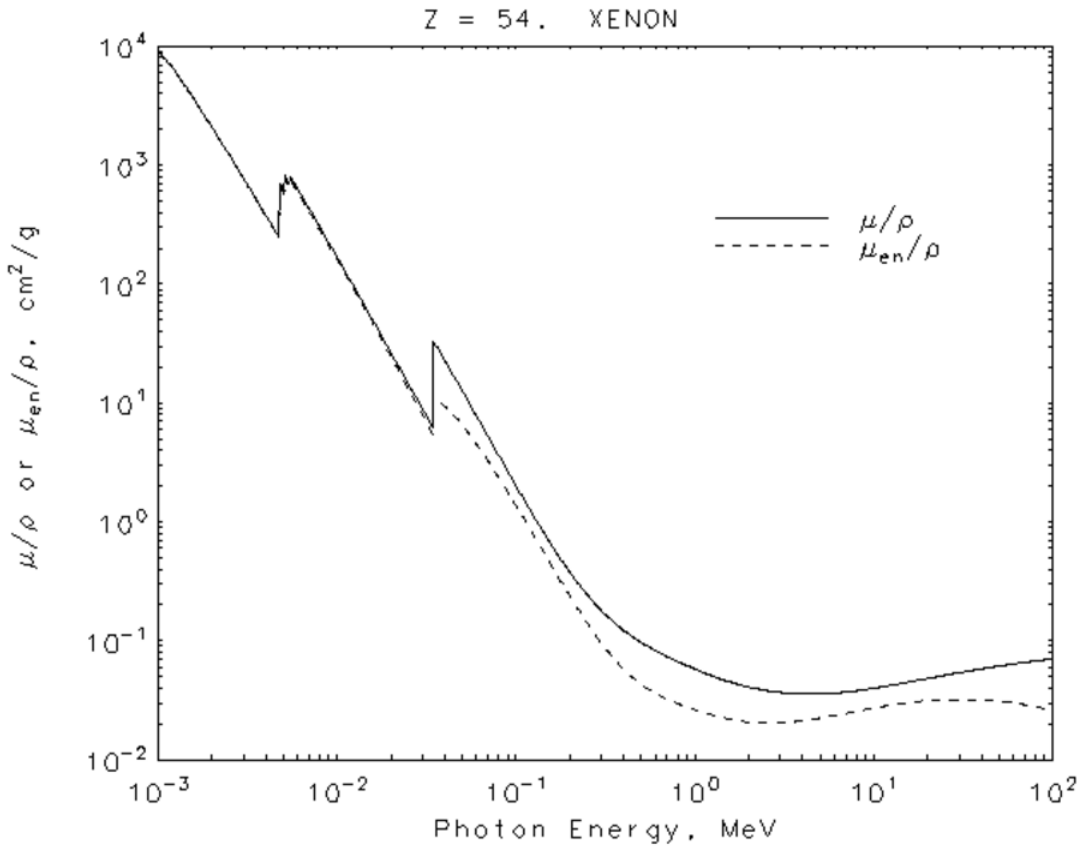
\includegraphics[width=\textwidth]{figs/NISTAttXenon.png}%  
		\mycaption[ The attenuation coefficient of xenon]{ The attenuation coefficient of xenon. The density of LXe is about 3\,g/cc, at the relevant temperature. }
		\label{fig:MFP}
		\end{center}
	
\end{figure} 

The calibration source needed should emit high energetic $\gamma$ photons and have a long half life so it will not need to be replaced. After careful examination of all available sources, a sealed \Th\ source was selected, see decay chain is in Fig.~\ref{fig:th228}. The energetic $\gamma$ emission line coming from $^{208}\mathrm{Tl}$ with energy of 2614\,keV and intensity of 0.99 can produce good calibration events, and the half life $t_{\sfrac{1}{2}}=1.9$\,years is long enough for operation.
The source is encapsulated inside SS, therefore all $\beta$ and $\alpha$ decay products will not reach the detector. Less energetic $\gamma$ emission lines will penetrate the Sensitive Volume (SV) and trigger the PMTs but will not proceed to the FV, therefore will be treated as ``background'', i.e., non-usable events.



\begin{figure}
	\begin{center}
	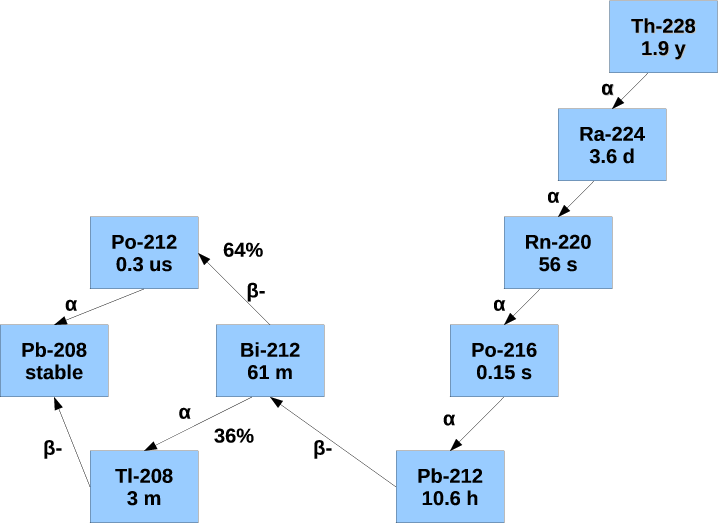
\includegraphics[height= 0.5\textheight]{figs/Th228Check.PNG}% Here is how to import 
		\mycaption[\Th\ decay chain]{ \Th\ decay chain }
		\label{fig:th228}		
		\end{center}
	
	\end{figure} 
 
In order to estimate the fraction of good calibration events from total triggering, all spectral lines are simulated.  
A summary of the more energetic $\gamma$ lines from \Th\ decay chain is presented in Table~\ref{table:isotope}.
\begin{table}
\begin{center}
\resizebox{0.75\textwidth}{!}{
 \begin{tabular}{||c c c ||} 
 \hline
 Energy (keV) & Isotope & Intensity \\ [0.5ex] 
 \hline 
  511 & $^{208}\mathrm{Tl}$ & 0.22 \\ 
 \hline
  583  & $^{208}\mathrm{Tl}$ & 0.85 \\
 \hline
 727 & $^{212}\mathrm{Bi}$ & 0.67 \\
 \hline
 763  & $^{208}\mathrm{Tl}$ & 0.18 \\
 \hline
  861  & $^{208}\mathrm{Tl}$ & 0.12 \\  
 \hline
  1621 & $^{212}\mathrm{Bi}$ & 0.15 \\  
 \hline
  2614  & $^{208}\mathrm{Tl}$ & 0.99 \\ 
 \hline
\end{tabular}
}
\caption{High energy $\gamma$lines from \Th\ decay chain}
\label{table:isotope}
\end{center}
\end{table}

All decays from $^{208}\mathrm{Tl}$ have an attenuation factor of 0.36 which is the branching ratio of $^{212}\mathrm{Bi} \rightarrow ^{208}\mathrm{Tl}$.
The fraction of 2614\,keV events interacting in the Sensitive Volume (SV) with respect to all events interacting in SV is 0.69.

\subsection{Charge Collection Efficiency (e$^-$ lifetime)}
The calibration of the charge collection efficiency is done with less strict data selection criteria than the ER band calibration. A good calibration sample  should have a well defined characteristic feature obtained from the source in various z-positions (e.g., full absorption peak). By comparing this feature dependency on height a charge collection efficiency map is produced. \Cs\ source which emits 662\,keV $\gamma$ photons and $t_{\sfrac{1}{2}} = 30$\,years, is selected for this calibration. The decay of \Cs\ is shown in Fig~\ref{fig:Cs}. The source is deposited inside a 25\,mm diameter disk. 


\begin{figure}
	\begin{center}
	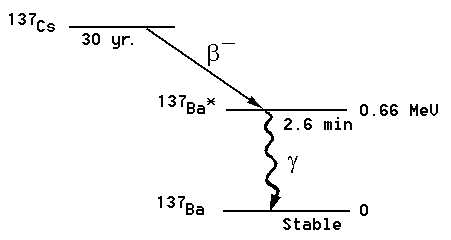
\includegraphics[width=0.55\textwidth, height= 0.3\textheight]{figs/Cs137.jpg}% Here is how to import 
		\caption{\label{fig:Cs} \Cs\ decay}
		\end{center}
	
	\end{figure} 

\section{Collimators} \label{sec:Col}
 
Large portion of the $\gamma$ photons arriving to the SV are scattered at the outskirts of the SV and do not reach the FV, these events trigger the PMTs; however they are of no use for ER band calibration. In order to lower this portion the $\gamma$ source is placed behind a frame, with a conical hole, such that the solid angle of the opening covers just the FV when the source is located at the height of the center of the TPC (see Fig. ~\ref{fig:Colimator}). 

 \begin{figure}
   \centering
    \begin{minipage}[c]{0.49\textwidth}
    \centering
    \subbottom[]{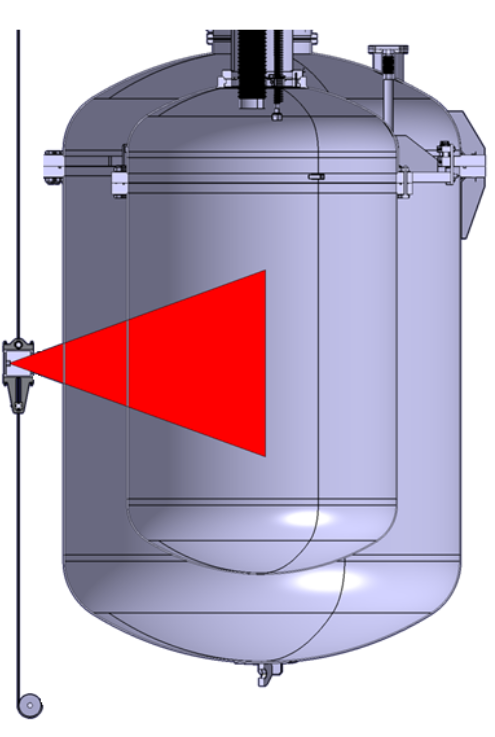
\includegraphics[width=\textwidth]{figs/collimator2.png}
%        \caption{The cryostat and the collimator shining just some of the FV }
        \label{subfig:colimator_cryo}}
    \end{minipage}
    \begin{minipage}[c]{0.4\textwidth}
	\centering    
        \subbottom[]{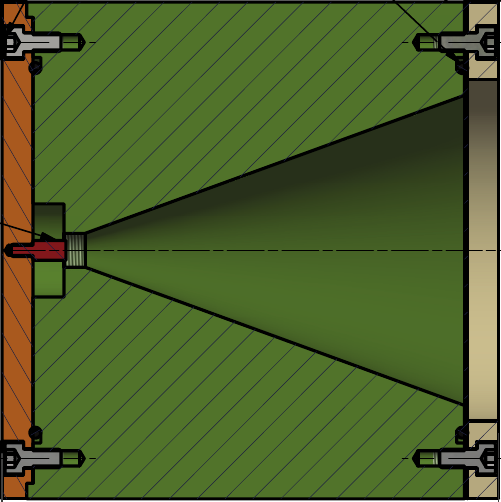
\includegraphics[width=\textwidth]{figs/CollimatorCAD.png}
%        \caption{a CAD design of the collimator with the conical hole.}
        \label{subfig:colimator_Cart}}
    \end{minipage} 
    \mycaption[ The cryostat and the collimator]{ (a) The cryostat and the collimator shining just part of the FV (b) a CAD design of the collimator with the conical hole. }
    \label{fig:Colimator}
\end{figure}

There are two types of collimators: a 16X16X16\,cm collimator which moves only vertically on a belt (I-Collimator), and a 10X10X10\,cm collimator which also passes below the cryostat (U-Collimator). 
Both collimators are made of Tungsten with a $45^{\circ}$ aperture, sealed with a 1\,mm SS plate to reduce the amount of water an emitted $\gamma$ travels through. 
The two collimators are designed to host both sources; the \Th\ source which has an M4 thread; and the disk \Cs\ source. An M12 thread is located in front of the source position to allow adding an attenuator, this can be done in parallel with detector operation.
 
The collimators are attached to belts that drive them to various calibration positions. The larger collimator is attached to the ``I-belt'', see Fig.~\ref{fig:IUBeltpic}. The smaller collimator is attached to the ``U-belt'', that passes below the cryostat, see Fig.~\ref{fig:IUBeltpic}. The two ``I-belts'' are connected to ports 5 and 11 while the ``U-belt'' is connected to ports 12 and 7, on the water tank's top flange, see Fig.~\ref{fig:topFlange}. The system allows integration with the sources and attenuators while the experiment is running, and modeling correctly quantities which may vary during the science run. 


\begin{figure}
	\begin{center}
	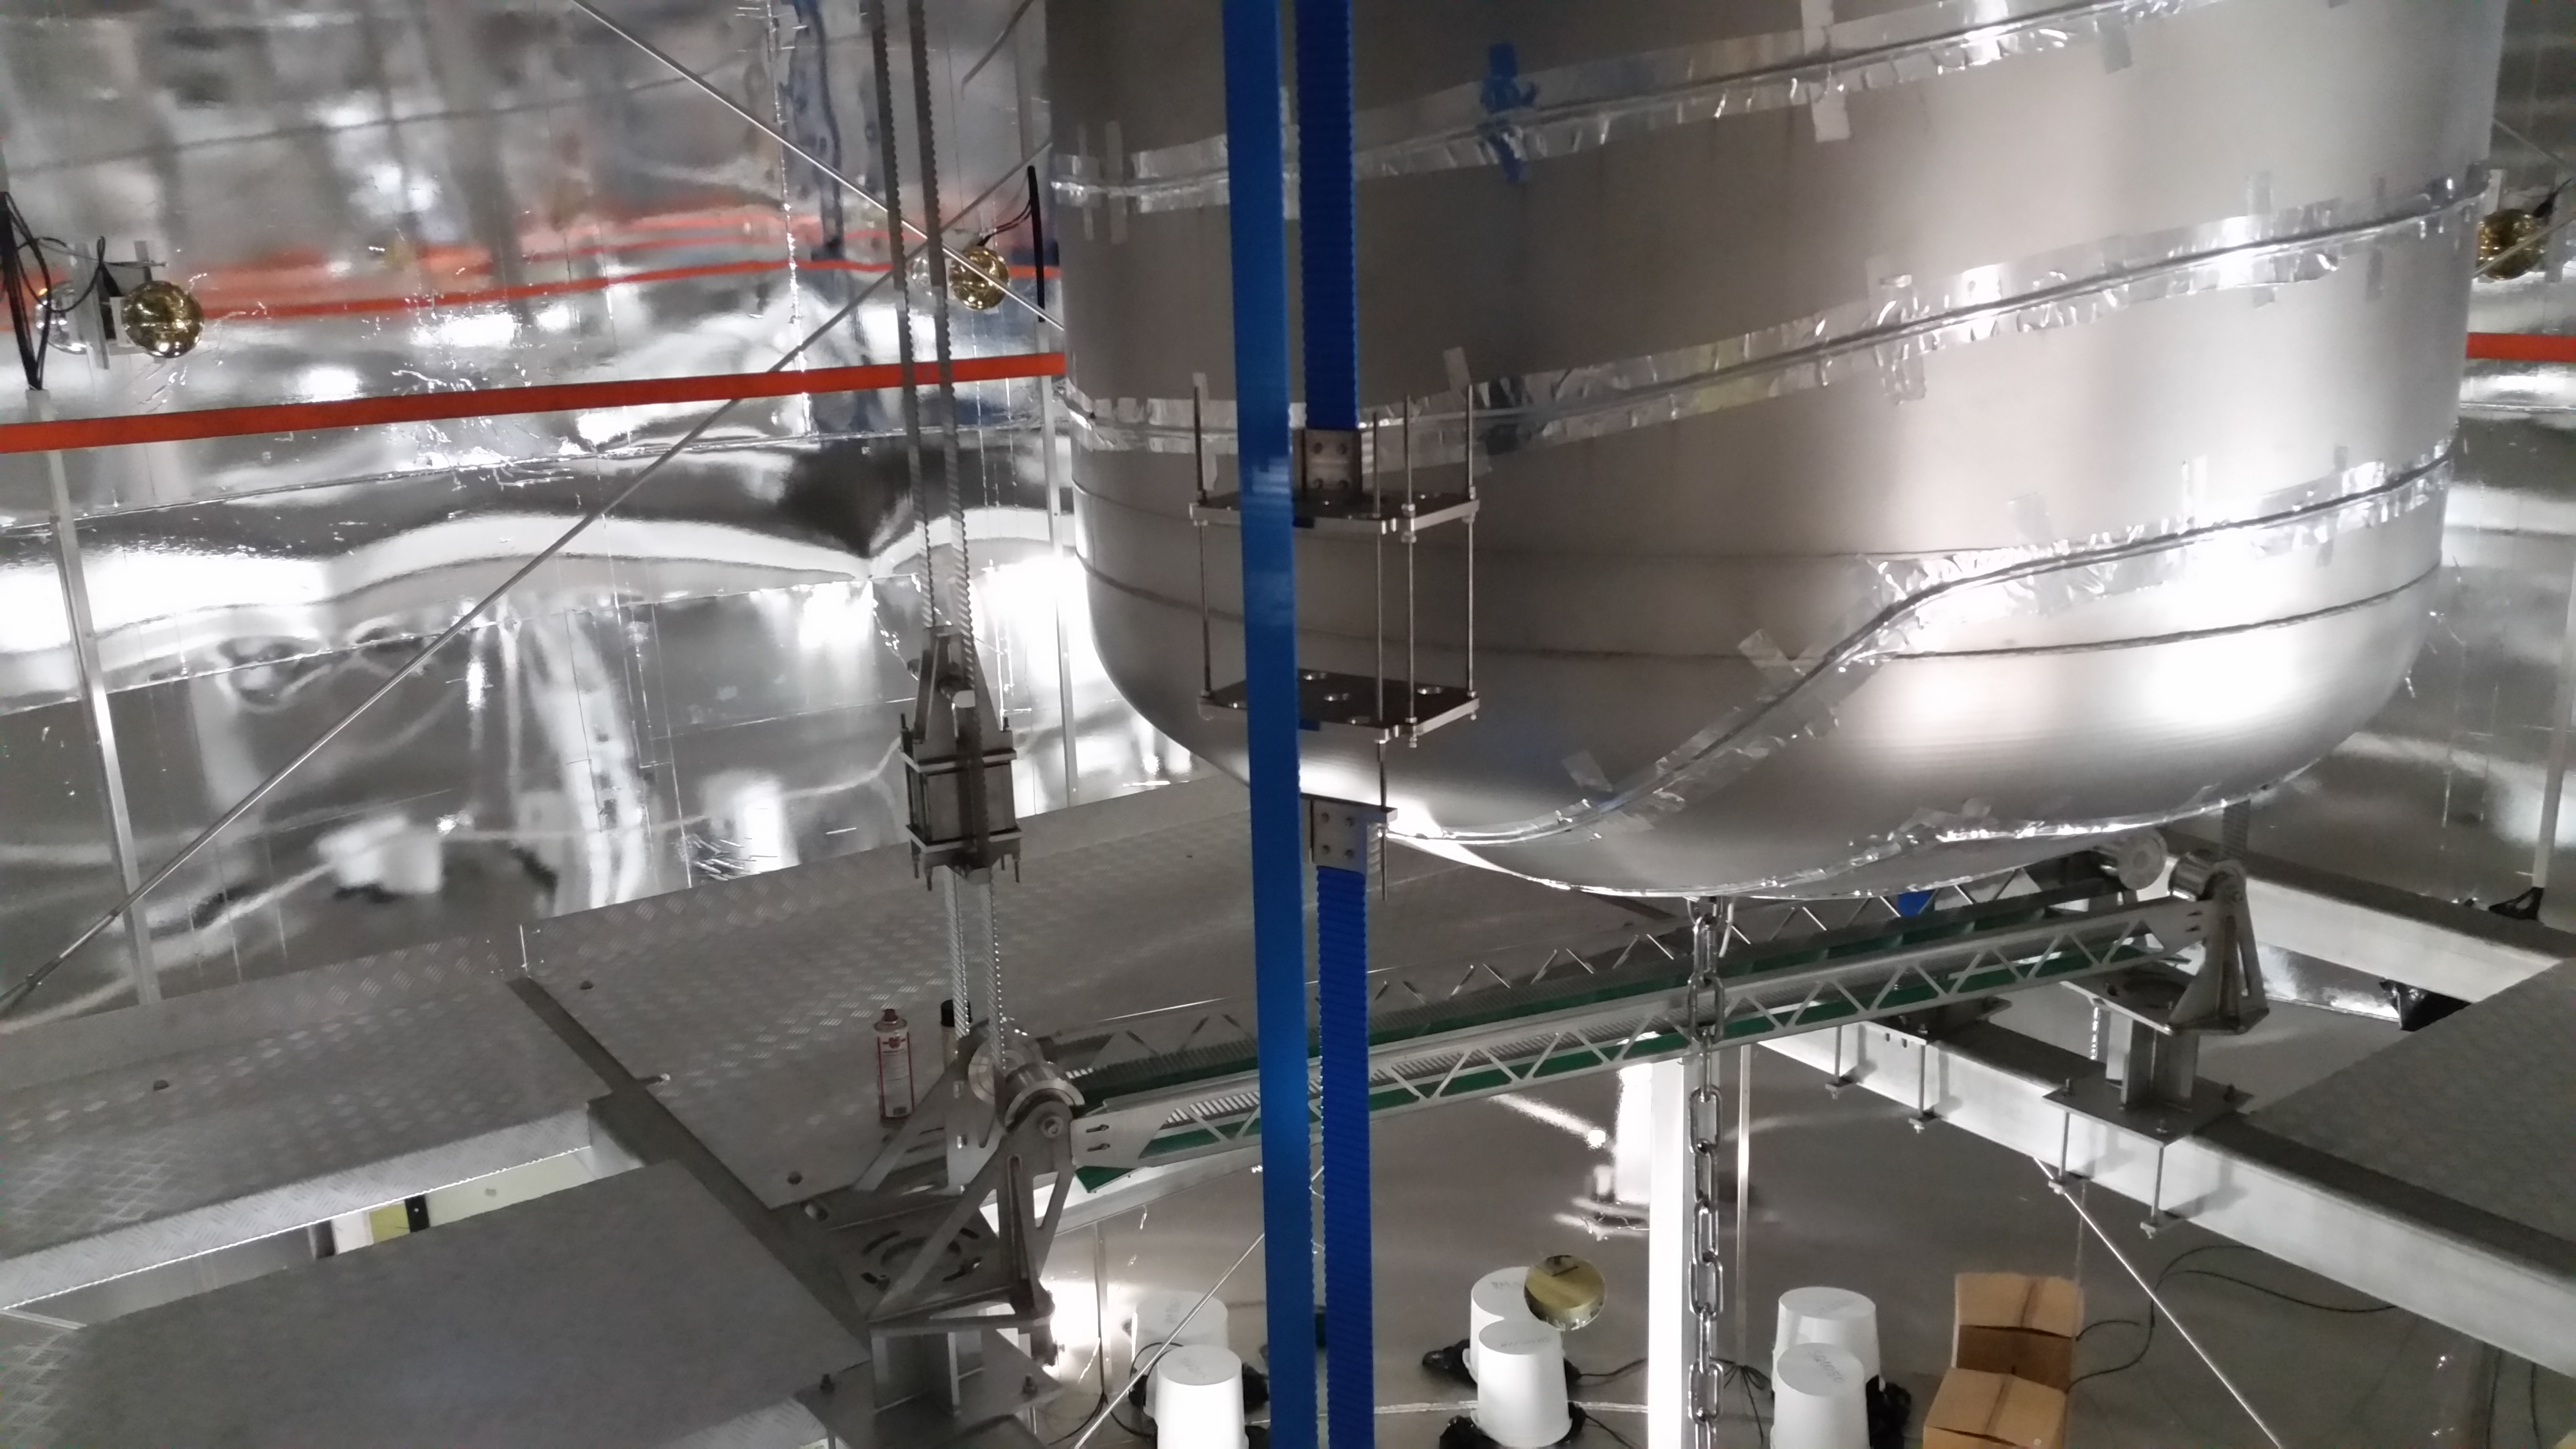
\includegraphics[width=\textwidth]{figs/IUBeltPic.jpg}% Here is how to import 
		\mycaption[A picture of the two belts]{A picture of the two belts. The blue belt is the I-Belt (currently not the I-Belt in use). The grey belt is the U-Belt (with the U-Collimator mounted), which passes below the cryostat.}
		\label{fig:IUBeltpic}
		
		\end{center}
\end{figure}



\begin{figure}
	\begin{center}
	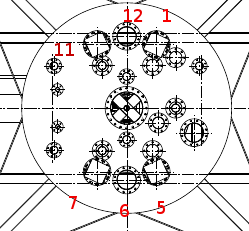
\includegraphics[width=0.55\textwidth]{figs/waterTankTopView.png}% Here is how to import 
		\caption{\label{fig:topFlange} A top view of the water tank }
		\end{center}
	
	\end{figure}
\subsection{Simulation} \label{subsec:simulation}

In order to decide the source activity and collimator design, MC simulations using the GEANT4 toolkit were used. The DAQ rate assumed for this study was 350\,Hz. Later it was realized that due to noise and purity conditions the benchmark rate should be, $\sim100$\,Hz. 

The results of the simulation of the final design of the I-Collimator which points to the center of the detector are shown in Table~\ref{table:ICol}, in Fig~\ref{fig:IBelt} are the original momentum-direction of $\gamma$ photons which do not produce a ``good'' calibration event. This is of importance to verify mainly events coming from the collimator opening will reach the detector's SV.


\begin{table}
\begin{center}
\resizebox{0.8\textwidth}{!}{
 \begin{tabular}{||c c||} 
 \hline
 number of simulated events & 2e9 \\ 
 \hline
 number of recorded events (SV) & 2.5e7 \\
 \hline
 number of good events & 53 \\
 \hline
 good evts/day @ 350Hz  & $65 \pm 8$ \\
 \hline
 evt/day after bkg reduction & 45 \\  
 \hline
\end{tabular}
}

\mycaption[result of GEANT4 simulations for a 16X16X16cm collimator]{result of GEANT4 simulations for a 16X16X16cm collimator with an aperture of $45 \deg$, a good event is an event that scattered only once in the FV with energy deposition of 2-15 keVee}
\label{table:ICol}
\end{center}
\end{table}


\begin{figure}
   \centering
    \begin{minipage}[b]{0.49\textwidth}
    \subbottom[]{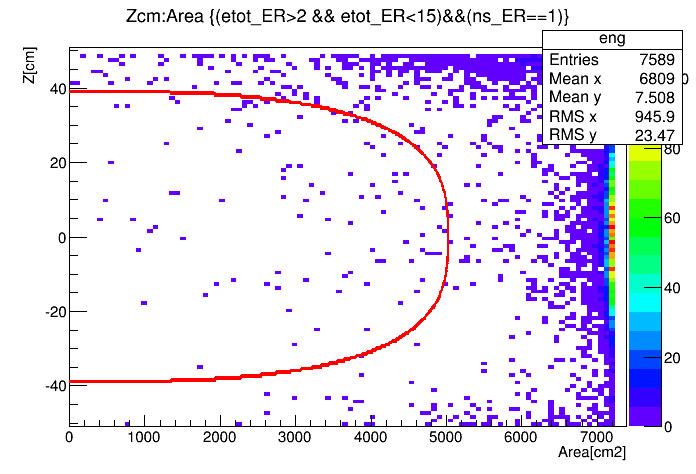
\includegraphics[width=\textwidth]{figs/scatter45deg16X16X16.png}
%        \caption{scatter of good calibration events in the SV, the red line is the border of the FV }
        \label{subfig:IBeltScatter}}
    \end{minipage}
    \begin{minipage}[b]{0.4\textwidth}
        \subbottom[]{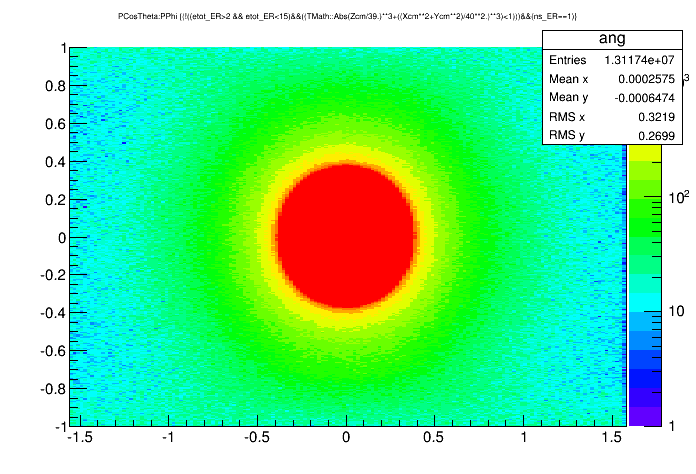
\includegraphics[width=\textwidth,height=0.23\textheight]{figs/angles16}
%        \caption{Intial momentom of background events i.e., events which trigger PMT's and do not meet all three conditions, FV, single scattered, and energy deposition range} 
        \label{subfig:IBeltAngle}}
    \end{minipage} 
    \mycaption[I-Collimator]{(a) scatter of good calibration events in the SV, the red line is the border of the FV  (b) Intial momentom of background events i.e., events which trigger PMT's and do not meet all three conditions, FV, single scattered, and energy deposition range 
}
\label{fig:IBelt}
\end{figure}



The \textsc{Xenon1T} cryostat  is attached by a spring to the water tank's floor, this is done to apply force against the detector's buoyancy while filling water. Therefore the ``U-belt'' cannot pass underneath the center of the detector. This causes the collimator to be in a small angle with respect to the center of the detector.
The results of the simulation of the U-Collimator are shown in table~\ref{table:UCol} and Fig.~\ref{fig:UBelt}. 



\begin{table}
\begin{center}
\resizebox{0.8\textwidth}{!}{
 \begin{tabular}{||c c||} 
 \hline
 number of simulated events & 4e9 \\ 
 \hline
 number of recorded events (SV) & 4.05e7 \\
 \hline
 number of good events & 58 \\
 \hline
 evt/day @ 350Hz good evts & $43 \pm 6$ \\
 \hline
 evt/day after bkg reduction & 30 \\  
 \hline
 Source activity & 80kBq \\ [1ex] 
 \hline
\end{tabular}
}
\mycaption[Result of GEANT4 simulation for a 10X10X10cm collimator]{Result of GEANT4 simulation for a 10X10X10cm collimator with an aperture of $45 \deg$, a good event is an event that scattered only once in the FV with energy deposition of 2-15 keVee}
\label{table:UCol}
\end{center}
\end{table}


\begin{figure}
   \centering
    \begin{minipage}[c]{0.49\textwidth}
    \subbottom[]{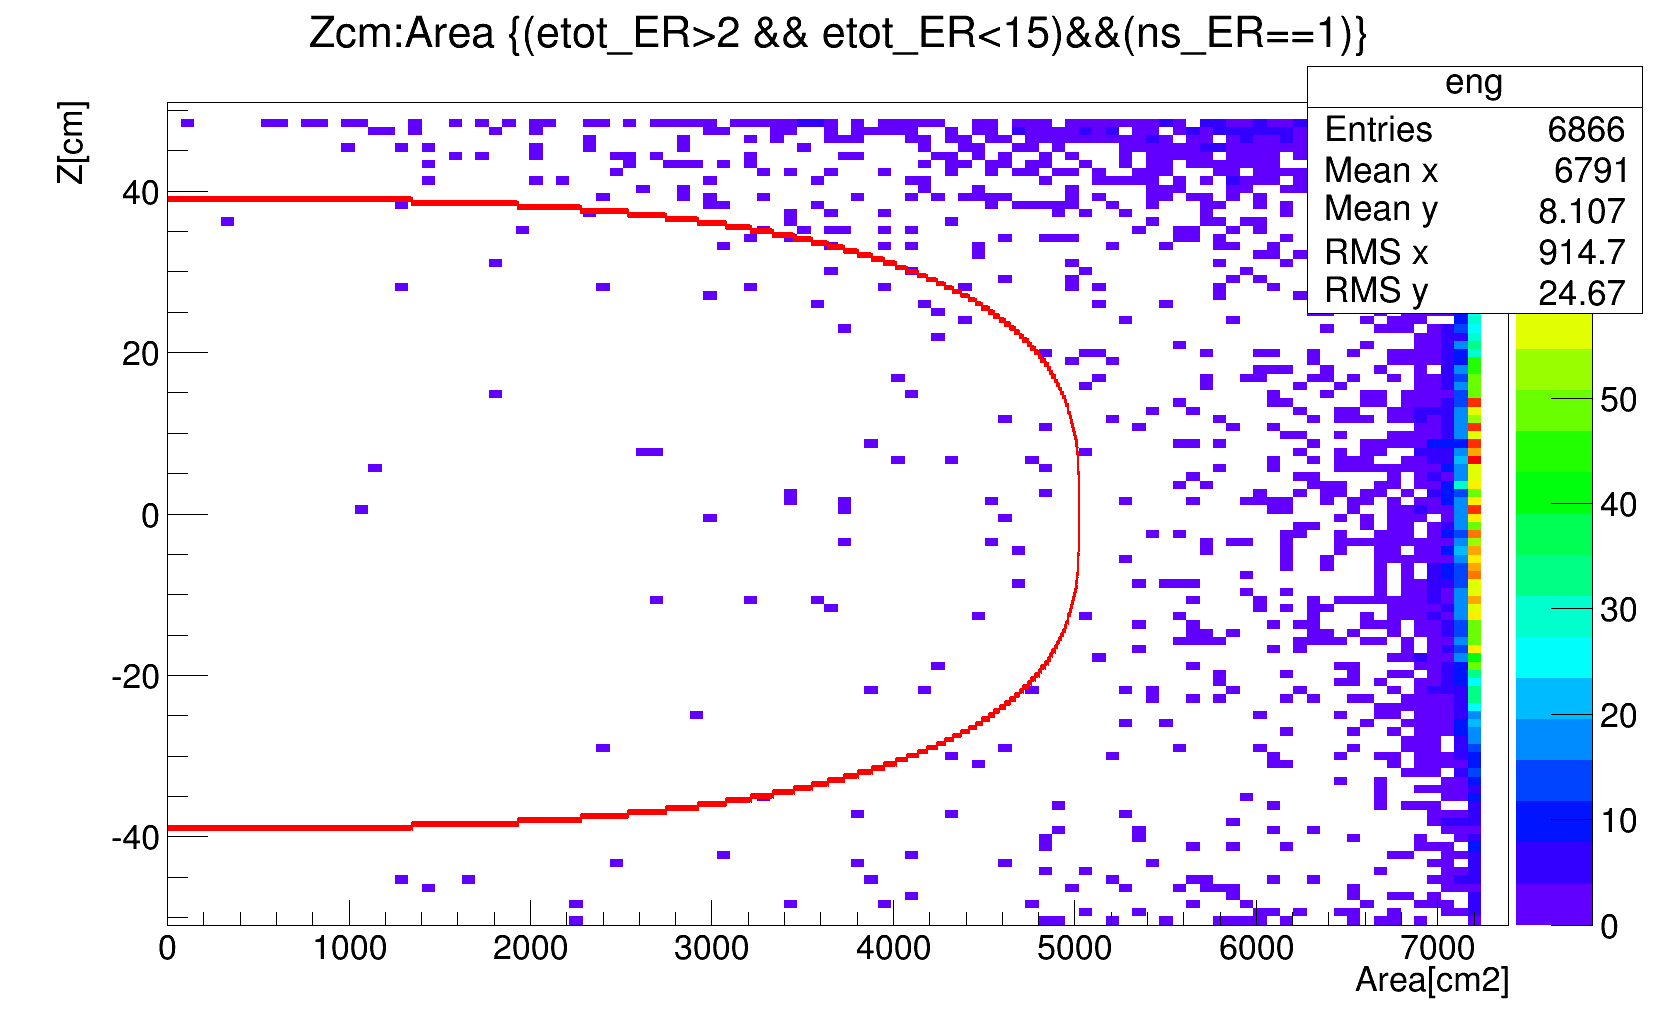
\includegraphics[width=\textwidth]{figs/ScatterPlot10X10X10NonCenteredSymetric.png}
%        \caption{scatter of good calibration events in the SV, the red line is the border of the FV }}
        \label{subfig:UBeltScatter}}
    \end{minipage}
    \begin{minipage}[c]{0.4\textwidth}
        \subbottom[]{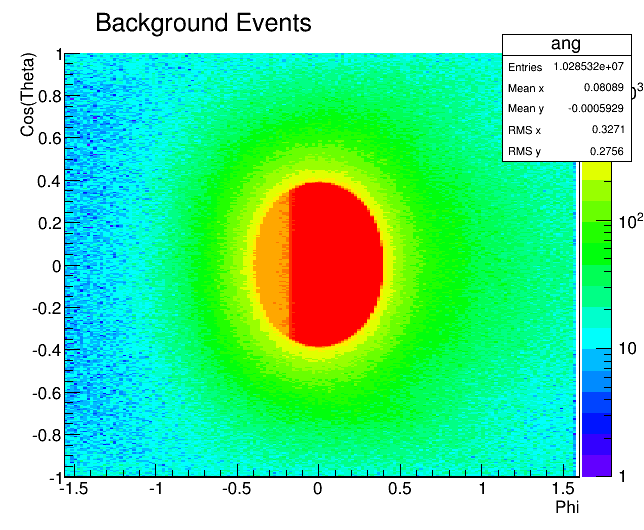
\includegraphics[width=\textwidth]{figs/Ang10X10X10NonCenteredSymetric.png}
%        \caption{Intial momentom of background events i.e., events which trigger PMT's and do not meet all three conditions, FV, single scattered, and energy deposition range} 
        \label{subfig:UBeltAngle}}
    \end{minipage} 
    \mycaption[U-Collimator]{(a) scatter of good calibration events in the SV, the red line is the border of the FV (b) Intial momentom of background events i.e., events which trigger PMT's and do not meet all three conditions, FV, single scattered, and energy deposition range 
}
\label{fig:UBelt}
\end{figure}

Comparing these results to early studies, simulating a ``bare'' source, show that using the collimators reduces the amount of time needed for calibration by a factor three. In addition the design allows sufficient flexibility.

During the first science run, a large population of events near the TPC walls was detected. Although these events were expected, the XY reconstruction and the energy deposition of them suggest that their might be a distortion to the electric field in large radii. In order to better understand the origin and quality of these events we are currently studying the possibility of reducing the intensity of the sources using an attenuator screwed into the designated place in the collimator and collecting data only from large radii.  

\section{Summary}

In this chapter I have presented the external calibration technique used in the \textsc{Xenon1T} detector. The radioactive sources used for different purposes are presented along with the collimators holding them. The collimators are attached to belt systems driving them to various positions. This technique reduces the calibration time by a factor of $\sim3$ with respect to naive calibration. The system is mounted and fully functional.   
